\subsection{Herstellung der Compact Disc}
\label{subsec:cdherstellung}

Die Herstellung einer CD beginnt mit der Anfertigung einer Glasmatrize. Diese
besteht aus einer Glasplatte und einer Fotolackschicht, welche die Pitstruktur
enthält. Aus dieser wird daraufhin eine Metallmatrize gefertigt, welche für das
Spritzgussverfahren verwendet wird. Dabei wird die Matrize in das flüssige
Polycarbonat gepresst. Dadurch überträgt sich die Pitstruktur, wie in
\autoref{fig:cdherstellung}, auf die Polycarbonatscheibe. Auf diese wird
anschließend das Aluminium aufgedampft, um die Reflexionsschicht zu erhalten,
und mithilfe einer Schutzschicht versiegelt. \cite{cdp}

\begin{figure}[h]
    \begin{center}
        \begin{minipage}[t]{\textwidth}
            \begin{center}
                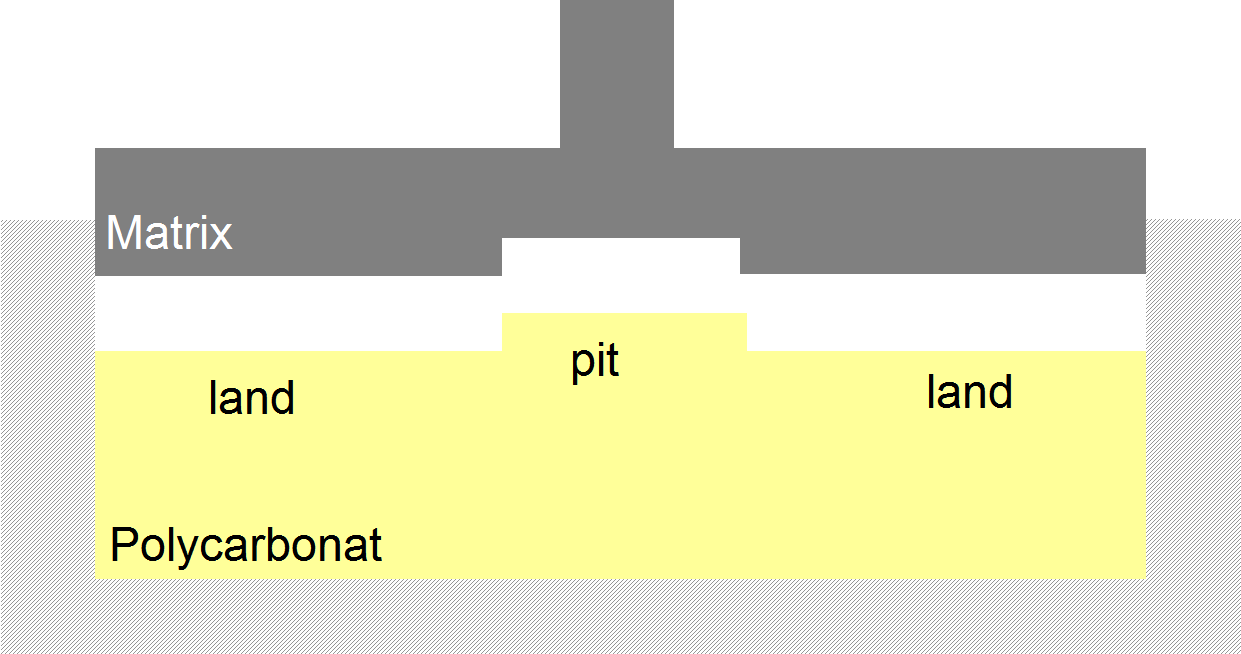
\includegraphics[height=0.1\textheight]{Bilder/Optische_Datentraeger_Die_Compact_Disc/Herstellung/cdherstellung.png}
                \caption[Übertragung der Pitstruktur \newline \url{http://daten.didaktikchemie.uni-bayreuth.de/umat/cd_dvd/spritzguss.gif} (zuletzt aufgerufen am 07.08.2015)]{Übertragung der Pitstruktur}
                \label{fig:cdherstellung}
            \end{center}
        \end{minipage}
    \end{center}
\end{figure}

Das Spritzgussverfahren selbst kann in drei Schritte unterteilt werden. Wie in
\autoref{fig:cdspritz} zu sehen beginnt der Vorgang des Plastifizierens mit dem
Einfüllen des zerkleinerten Polycarbonats (Granulat) in die Schnecke. Das
Granulate wird durch die Heizelemente und die sich drehende Schnecke
verflüssigt. Durch den an der Spitze aufgebauten Druck wird die Schnecke
teilweise aus dem Gehäuse (Plastifizierzylinder) herausgedrückt. Danach folgt
der Einspritzvorgang, dabei wird das geschmolzene Granulat durch die
Vorwärtsbewegung der Schnecke in die CD-Form und auf die Matrize gedrückt. Als
Letztes folgt das Abkühlen und Auswerfen der fertigen Polycarbonatscheibe.
\cite{cdpf}

\begin{figure}[h]
    \begin{center}
        \begin{minipage}[t]{\textwidth}
            \begin{center}
                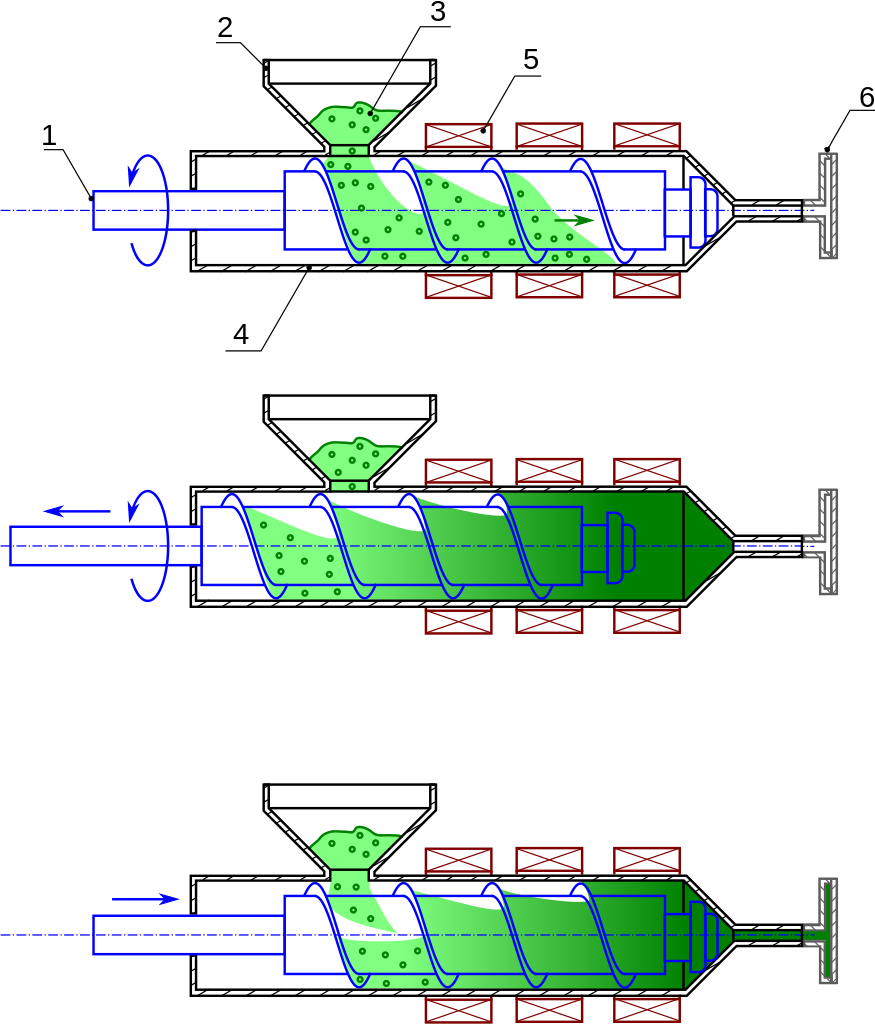
\includegraphics[height=0.5\textheight]{Bilder/Optische_Datentraeger_Die_Compact_Disc/Herstellung/cdspritz.png}
                \caption[Spritzgussverfahren \newline \url{https://upload.wikimedia.org/wikipedia/commons/thumb/2/23/Principe_moulage_injection_polymere.svg/899px-Principe_moulage_injection_polymere.svg.png} (zuletzt aufgerufen am 11.08.2015)]{Spritzgussverfahren: 1. Schnecke, 2. Einfülltrichter, 3. Granulat, 4. Plastifizierzylinder, 5. Heizelemente, 6. CD-Form inklusive Glasmatrize}
                \label{fig:cdspritz}
            \end{center}
        \end{minipage}
    \end{center}
\end{figure}
